\begin{thm}{050}{\hosi ?}{IMO (2017)}
 円$\Omega$上に$\mr{RS}$が直径とならない異なる2点$\mr{R, S}$があり、直線$\mr{RS}$上の点$\mr{T}$は$\mr{RS}=\mr{TS}$を満たす。劣弧$\mr{RS}$上に点$\mr{J}$をとる。$\Omega$の$\mr{R}$における接線と$\triangle\mr{JST}$の外接円$\Gamma$の交点のうち、$\mr{R}$に近い方を$\mr{A}$とすると、直線$\mr{AJ}$は点$\mr{K}$で再び$\Omega$と交わる。このとき、直線$\mr{KT}$は$\Gamma$に接することを示せ。
\end{thm}

まず、円$\Omega$の点$\mr{R}$における接線と円$\Gamma$の交点のうち、$\mr{R}$から遠いほうを点$\mr{B}$とし、直線$\mr{BJ}$と円$\Omega$との交点のうち$\mr{J}$でない方を点$\mr{L}$とする。

\begin{figure}[H]
 \centering
 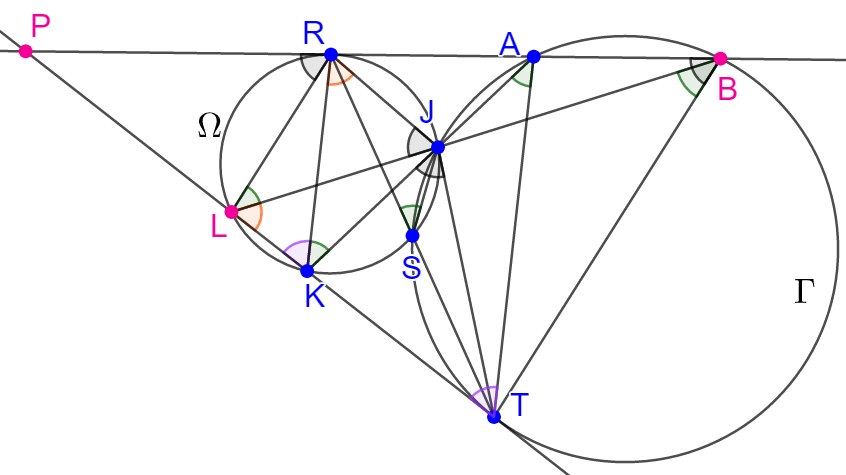
\includegraphics[width=0.8\linewidth]{../problems/Q_050/A_050.png}
\end{figure}

円周角の定理によって$\angle\mr{RKJ}=\angle\mr{RSJ}$であり、四角形$\mr{AJST}$が円$\Gamma$に内接することから$\angle\mr{RSJ}=\angle\mr{JAT}$である。よって$\angle\mr{RKJ}=\angle\mr{JAT}$となって、錯角が等しいから線分$\mr{RK}$と線分$\mr{AT}$は平行である($\cdots$ \marunum{1})。

円周角の定理によって$\angle\mr{RLJ}=\angle\mr{RSJ}$であり、四角形$\mr{BJST}$が円$\Gamma$に内接することから$\angle\mr{RSJ}=\angle\mr{JBT}$である。よって$\angle\mr{RLJ}=\angle\mr{JBT}$となって、錯角が等しいから線分$\mr{RL}$と線分$\mr{BT}$は平行である($\cdots$ \marunum{2})。

さて\marunum{1}によって同位角が等しいことから、$\angle\mr{RKL}=\angle\mr{ATK}$。また$\angle\mr{RKJ}=\angle\mr{JAT}$であったから、
\[ \angle\mr{JKL}=\angle\mr{RKL}+\angle\mr{RKJ}=\angle\mr{ATK}+\angle\mr{JAT} \]
が成り立つ。このことは、3点$\mr{T, K, L}$が1直線上にあることを示している($\cdots$ \marunum{3})。直線$\mr{RAB}$と直線$\mr{TKL}$の交点を$\mr{P}$とおく。

円周角の定理によって、$\angle\mr{JRK}=\angle\mr{JLK}$ ($\cdots$ \marunum{4})。

接弦定理によって、$\angle\mr{RJL}=\angle\mr{PRL}$。\marunum{2}によって同位角が等しいから、$\angle\mr{PRL}=\angle\mr{ABT}$。四角形$\mr{ABTJ}$が円$\Gamma$に内接することから、$\angle\mr{ABT}=\angle\mr{KJT}$。よって$\angle\mr{RJL}=\angle\mr{KJT}$であるから、
\[ \angle\mr{RJK}=\angle\mr{RJL}+\angle\mr{LJK}=\angle\mr{KJT}+\angle\mr{LJK}=\angle\mr{LJT} \]
が成り立つ。これと\marunum{4}によって$\triangle\mr{RJK}\sim\triangle\mr{LJT}$が示される。したがって、$\angle\mr{RKJ}=\angle\mr{LTJ}$となる($\cdots$ \marunum{5})。

最後に、$\angle\mr{RKJ}=\angle\mr{JAT}$であったから、\marunum{5}と合わせれば、$\angle\mr{LTJ}=\angle\mr{JAT}$となっている。円$\Gamma$において、接弦定理の逆によって直線$\mr{KT}$は円$\Gamma$の接線であることが示された。\footnote{なお、ここまでの議論で$\mr{RS}=\mr{TS}$の条件を使っていないように見えるが、これが満たされていないと題意の図は構成されない。本証明の中でどのように暗に含まれているかは実は未解決。また、点$\mr{R}$における円$\Omega$の接線が円$\Gamma$にも接する場合には、直線$\mr{KT}$は円$\Gamma$だけでなく円$\Omega$にも接する。}